
\section{Cellular automata}
Lattice Gas Cellular Automata (LGCA) has different restrictions which simplify our computations and decrease the computation costs,in contrast to MD. For example, intermolecular forces are replaced with rigid body collisions, and during one time step particles can travel only along one edge. The velocities are discretized too, which implies that all particles have the same energy and at the end of a time step particles can only reside at the vertices.

The first lattice-gas cellular automata (LGCA) was proposed in 1973 by Hardy, de Pazzis and Pomeau [3]. It is named HPP and is a LGCA model over square lattice. HPP does not lead to Navier-Stokes equations, because of insufficient degree of rotational symmetry of the lattice. But still it is worth  discussing, and  will be done later on.

Frish-Hasslacher-Pomeau is the model of LGCA (see Fig. 1), which leads to Navier-Stokes equations, because of its symmetry. For example Frish-Hasslacher-Pomeau automata has following prescriptions [2]:


\begin{itemize}
\item All particles have the same mass m=1.
\item Particles can move only along one of the six directions defined by the discrete displacements $c_{i}$.
\item In a time-cycle (made one for convenience) the particles hop to the nearest neighbor pointed by the corresponding discrete vector $c_i$. Both longer and shorter jumps are forbidden, which means that all lattice particles have the same energy.
\item No two particles sitting on the same site can move along the same direction $c_{i}$ (exclusion principle).
\end{itemize}

\begin{figure}[H]
  \centering
  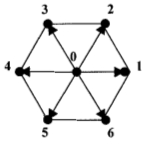
\includegraphics[width=0.1\textwidth]{img/fig1.png}
  \caption{The FHP hexagonal lattice [2].}
\end{figure}

LGCA exhibits the following basic mechanisms:

\begin{itemize}
\item Free-streaming: $ n_i^{in}(\vec{r}+\vec{c}_{i}\Delta t, t+\Delta t) = n_i^{out}(\vec{r}, t) $
\item Collision: $ n_i^{out}(\vec{r}, t) = n_i^{in}(\vec{r}, t) + \Omega(n_i^{in}(\vec{r}, t)) $.
\end{itemize}
Where $\Omega$ is a collision operator.

Free-streaming is a simple transfer of particles according to their discrete velocities.

When two particles meet each other on the site they interact and exchange their momenta following the discretization rules of the lattice. Such exchange is called collision. In HPP only two particles can collide, that is why the collision in HPP is deterministic (see Fig. 2a).

If  the collision of two particles in FHP is considered, then the outcome will be non-deterministic (see Fig. 2b).

\begin{figure}[H]
  \centering
  \begin{subfigure}[h]{0.5\textwidth}
    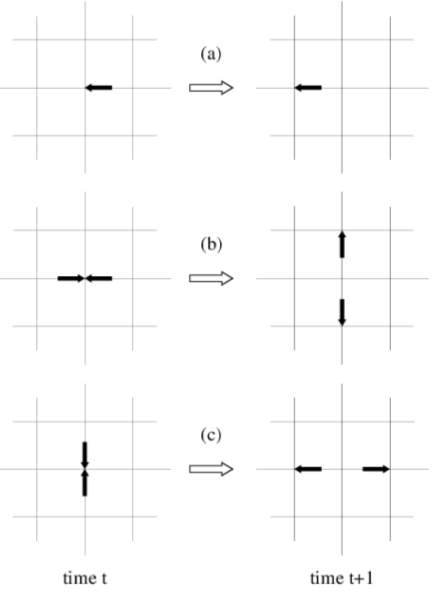
\includegraphics[width=\textwidth]{img/fig4.png}
    \caption{HHP streaming(a)/collision(b,c) [6].}
  \end{subfigure}
  \begin{subfigure}[h]{0.3\textwidth}
    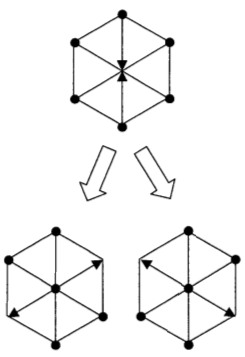
\includegraphics[width=\textwidth]{img/fig5.png}
    \caption{FHP collision [2].}
  \end{subfigure}
  \caption{Collision of two particles / streaming.}
\end{figure}

Despite all the restrictions, this collision shares two crucial features such as conservation of particle number and conservation of the total momentum.

\begin{itemize}
\item conserve mass (number of particles): $ \sum_i n_i^{in} = \sum_i n_i^{out} $
\item conserve momentum: $ \sum_i n_i^{in} \vec{c}_{ia} = \sum_i n_i^{out} \vec{c}_{ia} $
\end{itemize}

One of the biggest advantages of LGCA is its easy implementation, and the ease
of its parallelization, because of local behaviour of the collision operator.

But the discretization doesn’t always work. For Macro-view such discretization is not a big problem, because discretization is always done, but for Micro-view such restrictions can lead to huge inconsistency and very poor precision. Restrictions in velocity direction and magnitude cannot describe a model at a microscopic level. LGCA includes the state of the particle where the velocity is equal to zero (stationary particles), but in real world these particles can not exist at the microscopic level. There are several main drawbacks of LGCA [3], but the most important one is statistical noise.

Lattice-Boltzmann approach was created as a response to the main problems of LGCA,using a statistical averaging procedure.
